 \section{Mappings} \label{sec:mappings}
Fran\c{c}ois Faure

% % mappings
\newcommand{\JNL}{\ensuremath{\mathcal{J}}}     % positions
\newcommand{\J}{\ensuremath{J}}     % mapping lineaire

\newcommand{\mass}{\ensuremath{M}}             % matrice de masse
\newcommand{\vol}{\ensuremath{\mathcal V}} % volume d'intersection
\newcommand{\press}{\ensuremath{\rho}}

% In section~\ref{sec:pixelcontact}, we have shown how to efficiently compute repulsion forces between arbitrary polyhedra.
% In this section, we present a general framework to map the contact forces to the degrees of freedom of arbitrary physical models.
% We then demonstrate it on a variety of models.

\subsection{Geometrical layers} \label{sec:geometryLayers}
Different geometrical models are used to model objects in contact.
We organize them in a hierarchy of layers. An example is shown in figure~\ref{fig:hierarchy}, where a rigid object hits a shape embedded in deformable cells.

\begin{figure}
 \centering
 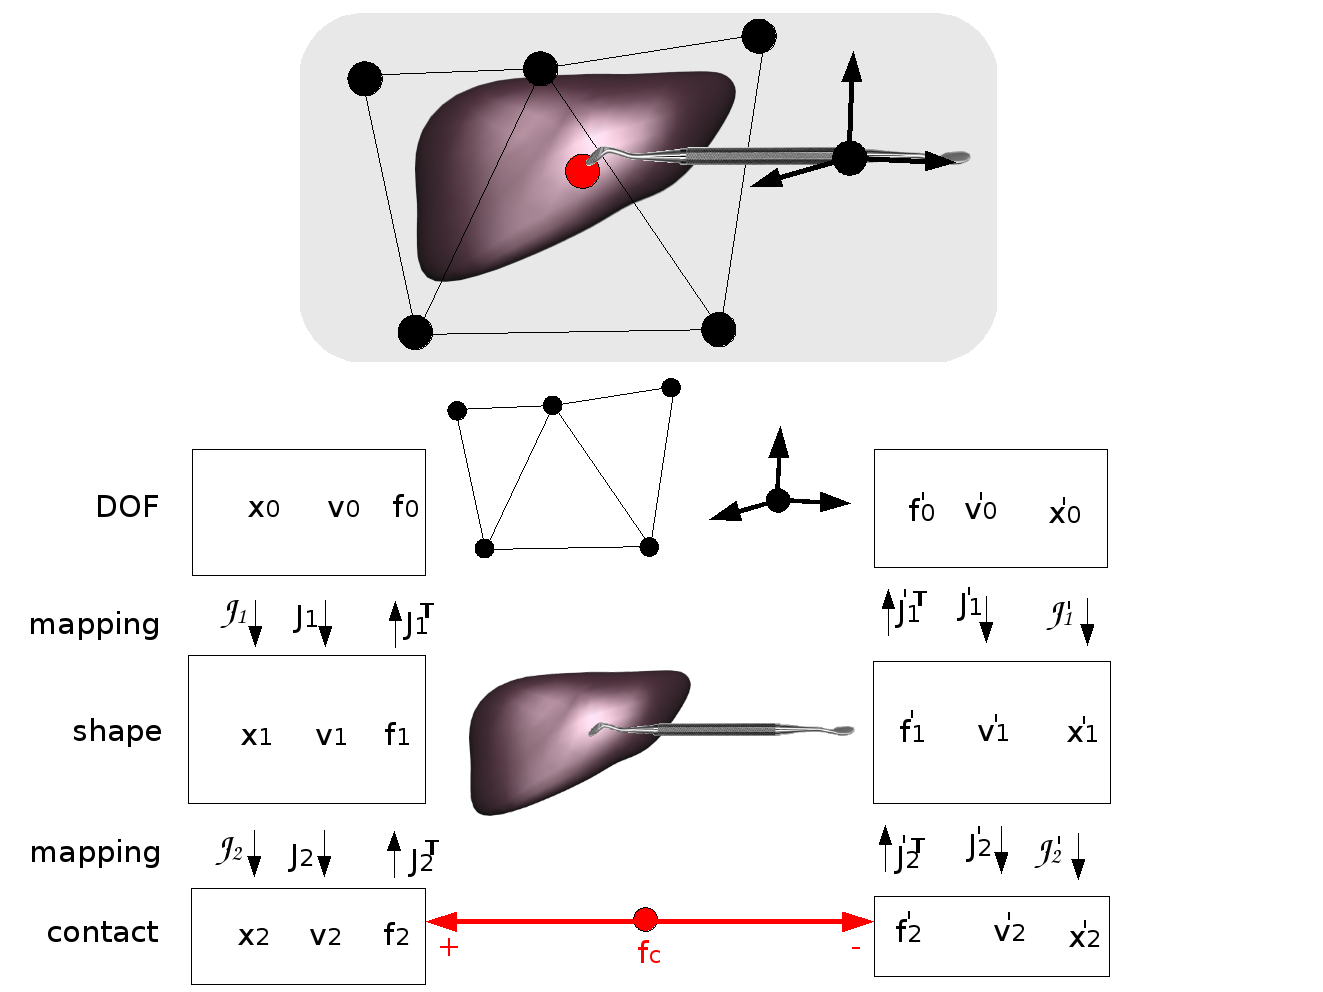
\includegraphics[width=\linewidth]{mappings.png}
 \caption{Mappings from the DOFs to a contact point. Top: two simulated objects in contact (red point). Bottom: hierarchy of geometrical layers. Positions and velocities are propagated top-down. The contact force $f_c$ is accumulated in the contact layers. Forces are then propagated bottom-up.
%Each object has its own state vectors and mappings.
}
 \label{fig:hierarchy}
\end{figure}

% bases de la dynamique
The state of a simulated system can be described by the values and time derivatives of its independent degrees of freedom (DOF) gathered in two vectors $x_0$ and $v_0$.
The dynamics equation (Newton's law) relates the second time derivative $a_0$ of the DOF to the forces $f_0$ acting on them: $f_0 = \mass a_0$, where \mass~ is a matrix modeling the mass of the system.
%We call $f_0$ the \textit{net force}.

% attacher de la g�om�trie
Geometry can be attached to the DOF for visualization or contact computation. 
We call it the \textit{shape}.
It is typically defined by points, such as triangle vertices or sphere centers, and additional data such as triangle connectivity or sphere radii.
We call these points the \textit{vertices}. 
Their positions, velocities and associated forces are stored in vectors $x_1$, $v_1$ and $f_1$, respectively.
They are not independent variables, since the positions and velocities are bound to the DOF using kinematic operators which we call the \textit{mappings}:
\begin{eqnarray*} %\label{eq:mapV}
x_1 &=&\JNL_1(x_0)\\ 
v_1 &=& J_1 v_0
\end{eqnarray*}
When the vertices and the DOF are the same, the mapping is the identity.
This special case occurs for instance when we simulate cloth or rigid balls.
More general cases include polygonal shapes attached to rigid bodies using local coordinates, or embedded in deformable cells using barycentric coordinates, as well as skin surrounding articulated bodies using vertex blending techniques.
Matrix $J_1 = \frac{\partial x_1}{\partial x_0}$ encodes the linear relation between the DOF velocities and the shape velocities. Due to linearity, the same relation holds on elementary displacements $dx$.
It also holds on accelerations, with an additional offset due to velocities when the position mapping \JNL is nonlinear.
In most cases, operators \JNL~ and \J~ are the same, but in the case of rigid bodies, \JNL~ is nonlinear with respect to $x$ and it can not be written as a matrix.
For surfaces embedded in deformable cells, matrix \J~contains the barycentric coordinates. 
For surfaces attached to rigid bodies, each row of the matrix encodes the usual relation $v = \dot o + \omega \times (x-o)$ for each vertex. 
Similarly, skins around articulated bodies involve, at each vertex, the weighted  contributions of the rigid bodies. 


% g�om�trie suppl�mentaire d�e aux contacts
When shapes collide, additional geometry can be necessary to model the contact.
For instance, when an edge intersects another one, a contact force is applied to the intersection points.
These points are defined by their barycentric coordinates with respect to their edge vertices. Other relations can be used, depending on the kind of geometrical primitives in contact.
This additional geometry requires another geometrical layer connected to the shape by a mapping, as illustrated in figure~\ref{fig:hierarchy}.
% This layer is also connected to the shape using mappings:
% \begin{eqnarray*} %\label{eq:mapV}
% x_2 &=&\JNL_2(x_1)\\ 
% v_2 &=&J_2 v_1 
% \end{eqnarray*}

We can straightforwardly extend this approach to tree-like hierarchies of geometries, with the DOF layer at the root. 
For instance, the DOF layer may have two independent children, one for collision using a coarse mesh, and the other for rendering using a finer mesh. The synchronization between these sibling layers is automatically guaranteed by their attachment to their common ancestor, the DOF layer.
The hierarchy can also be deeper, using for instance a fine mesh for rendering and its convex hull for collision.
This flexible framework gives us a great freedom for physical modeling.

\subsection{Mechanical mappings}
Positions and velocities can be propagated top-down through our layer hierarchy using the relations presented in the previous section.
In order to take the contact forces into account in the dynamics equation, we have to convert the contact forces applied to the contact points to forces applied to the DOF, where Newton's law is applied. 
This requires an extension to the position and velocity mappings presented in section~\ref{sec:geometryLayers}. We call it \textit{mechanical mapping}.

We derive a new, general method to propagate forces bottom-up through the layers of the geometrical hierarchy.
Given forces $f_n$ applied to a geometry layer $n$, we derive the equivalent force applied to its parent layer $n-1$. 
Equivalent forces must have the same power. Thus, we have to compute $f_{n-1}$ such that:
$$
v_{n-1}^T f_{n-1} = v_n^T f_n
$$
The relation $v_{n} = J_{n}v_{n-1}$ allows us to rewrite the previous equation as
$$
v_{n-1}^T f_{n-1} = v_{n-1}^T J_{n}^T f_n
$$
Since this relation must hold for any velocity $v_{n-1}$, we simplify it and get
\begin{equation} \label{eq:mapF}
f_{n-1} = J_n^T f_n
\end{equation}
This corresponds to the principle of virtual work.
%This simple relation allows us to map forces bottom-up through the hierarchy. 
%The corresponding acceleration can then be computed in the DOF layer.

% We emphasize the simplicity and the generality of equation~\ref{eq:mapF}. 
% It makes no assumption about the constitutive laws of the simulated objects.
% It allows us to connect arbitrary bodies using any geometry, provided that a kinematic operator linking the velocity of the geometry to the body DOFs is available.
% %It is not limited to polygonal geometries.
% It encompasses and generalizes \cite{Sifakis07}'s hard bindings which were introduced for Finite Elements and empirically extended to rigid bodies.
% It enables us to efficiently and straightforwardly connect or make collide a wide variety of bodies.


